\documentclass[UTF8,12pt,a4paper]{ctexart}

\usepackage{amsmath}
\usepackage{cases}
\usepackage{cite}
\usepackage{graphicx}
\usepackage{enumerate}
\usepackage{algorithm}
\usepackage{caption}   % \caption*需要
\usepackage{subcaption} % 子图布局
\usepackage[noend]{algpseudocode} %algorithmicx
\makeatletter
\renewcommand{\fnum@algorithm}{\fname@algorithm}
\makeatother
\renewcommand{\algorithmicrequire}{\textbf{Input:}}
\renewcommand{\algorithmicensure}{\textbf{Output:}}
\usepackage[margin=1in]{geometry}
\geometry{a4paper}
\usepackage{fancyhdr}
\pagestyle{fancy}
\fancyhf{}
\usepackage{xcolor}

% ------------------- 设置超链接,便于跳转 -----------------
\usepackage{enumitem}
\usepackage{hyperref}
\hypersetup{
    pdfborder={0 0 0},    % 消除超链接边框
    colorlinks=true,       % 将边框改为颜色标记(可选)
    linkcolor=black,       % 内部链接颜色(目录、引用等)
    citecolor=black,       % 引用颜色
    urlcolor=blue          % URL链接颜色(保持蓝色以便区分)
}

% ------------------- 三线表所需宏包 --------------------
\usepackage{booktabs} % 在导言区添加

% ------------------- 自定义代码展示风格 -----------------
\usepackage{listings}
\usepackage{xcolor}
\lstdefinestyle{hspice}{
    language=C,
    basicstyle=\ttfamily\small,
    keywordstyle=\color{blue}\bfseries,
    commentstyle=\color{green!50!black},
    stringstyle=\color{brown},
    numbers=left,
    numberstyle=\tiny\color{gray},
    stepnumber=1,
    numbersep=5pt,
    backgroundcolor=\color{white},
    showspaces=false,
    showstringspaces=false,
    showtabs=false,
    frame=single,
    rulecolor=\color{black},
    tabsize=2,
    captionpos=b,
    breaklines=true,
    breakatwhitespace=true,
    escapeinside={\%*}{*)},
    morekeywords={param, include, temp, option, probe, DC, dc, measure, alter, VDD, GND, gnd, NMOS, PMOS,FIND, WHEN, sweep, abs, I, SUPPLY, lg, fin_height, fin_width, tran, ac, op, model, end, subckt,ends,global, nmos, pmos, inv, data, +}, % 根据需要添加更多HSPICE关键字
    comment=[l]{*} % 在这里设置注释
}

\lstset{style=hspice} % 只应用样式


% ------------------------ 标题区 ----------------------------
\title{DIC Lab2 Report}
\author{
	Name: \underline{Jun Feng}~~~~~~
	ID: \underline{523031910148}~~~~~~}
\date{\today}
\pagenumbering{arabic}

\begin{document}



% ------------------------ 页眉和页脚 ----------------------------
\fancyhead[L]{Jun Feng}
\fancyhead[R]{DIC Lab2}
\fancyfoot[C]{\thepage}

\maketitle
\tableofcontents
\newpage
\section{Introduction and Background}

This report presents the results of Digital Integrated Circuit Lab 2, focusing on the analysis and optimization of CMOS inverter chains using FinFET technology. The primary objectives of this laboratory are:

\begin{itemize}
    \item Measurement and characterization of inverter delay parameters (FO4 delay)
    \item Optimization of multi-stage inverter chains for minimum delay
    \item Power consumption analysis of optimized inverter chains
    \item Energy-Delay Product (EDP) optimization through supply voltage scaling
    \item Investigation of optimal stage number selection for inverter chain design
\end{itemize}

The experiments utilize HSPICE simulation with 16nm FinFET technology models. FinFET technology offers superior electrostatic control and reduced short-channel effects compared to traditional planar MOSFETs, making it suitable for advanced technology nodes. Throughout this lab, we explore fundamental trade-offs in digital circuit design, including the relationship between delay, power consumption, and energy efficiency.

The inverter chain optimization problem is particularly important in practical circuit design, where signals must drive large capacitive loads through multiple stages. By carefully selecting the number of stages and the sizing factor of each stage, we can minimize propagation delay while maintaining acceptable power consumption.

\newpage
\section{Task 1: FO4 Delay Measurement}

\subsection{Lab Procedures}

The objective of Task 1 is to measure the Fan-Out-4 (FO4) delay of an inverter, which is a fundamental metric for characterizing the speed of a technology. The FO4 delay represents the propagation delay of an inverter driving four identical copies of itself.

The measurement setup consists of a chain of inverters where each inverter drives the next stage. HSPICE simulation is performed with the following key steps:

\begin{enumerate}
    \item[1. ] Define an inverter subcircuit using FinFET models
    \item[2. ] Create a chain of inverters with proper fan-out configuration
    \item[3. ] Apply a pulse input signal to the first stage
    \item[4. ] Measure the propagation delay \textbf{at the third inverter output}
    \item[5. ] Calculate both high-to-low ($t_{pHL}$) and low-to-high ($t_{pLH}$) delays using ".measure" statements
\end{enumerate}

The measurement statements in HSPICE trigger on the 50\% point of the supply voltage (0.5*SUPPLY) to accurately capture the propagation delay:

\begin{lstlisting}
.measure tran tpLH TRIG V(in) = 0.5*SUPPLY FALL = 2 TARG V(out) = 0.5*SUPPLY RISE = 2
.measure tran tpHL TRIG V(in) = 0.5*SUPPLY RISE = 2 TARG V(out) = 0.5*SUPPLY FALL = 2
.measure tran tp param='(tpLH+tpHL)/2'
\end{lstlisting}

\subsection{Lab Results}

The simulation results for the third inverter in the chain show the following delay characteristics \ref{tab:task1_results}:

\begin{table}[h]
\centering
\begin{tabular}{cccc}
\toprule
\textbf{Parameter} & \textbf{Value (ps)} & \textbf{Temperature (°C)} & \textbf{Alter \#} \\
\midrule
$t_{pLH}$ & 6.190 & 25.0 & 1 \\

$t_{pHL}$ & 5.633 & 25.0 & 1 \\

$t_p$ & 5.911 & 25.0 & 1 \\
\bottomrule
\end{tabular}
\caption{Measured FO4 delay parameters}
\label{tab:task1_results}
\end{table}

The waveform plots demonstrating the delay measurements are shown in Figures \ref{fig:task1_tphl} and \ref{fig:task1_tplh}.

\begin{figure}[htbp]
    \centering
    % 第一张子图
    \begin{subfigure}[b]{0.45\textwidth} % 子图宽度为总宽度的45%
        \centering
        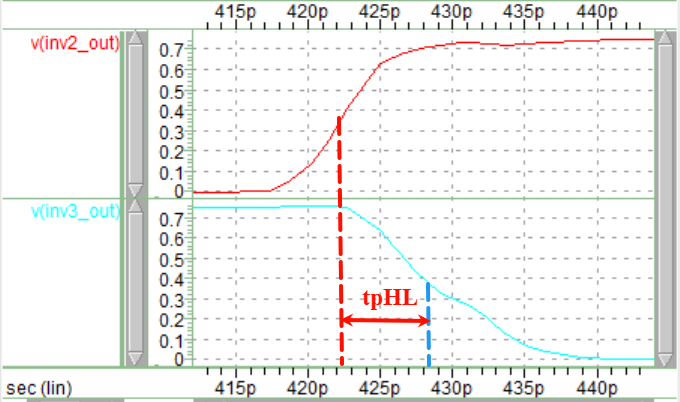
\includegraphics[width=\textwidth]{任务书/image.png} 
        \caption{$t_{pHL}$ measurement waveform(for illustration only)}
        \label{fig:task1_tphl}
    \end{subfigure}
    \hfill % 添加水平间距
    % 第二张子图
    \begin{subfigure}[b]{0.45\textwidth}
        \centering
        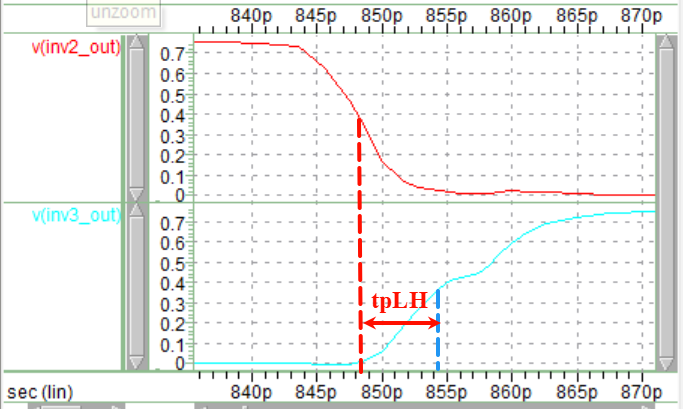
\includegraphics[width=\textwidth]{任务书/image-1.png} 
        \caption{$t_{pLH}$ measurement waveform(for illustration only)}
        \label{fig:task1_tplh}
    \end{subfigure}
    % 总图标题
    \caption{$I_{\text{DS}}-V_{\text{DS}}$ curve}
    \label{fig:task1_waveform}
\end{figure}
\subsection{Technical Analysis}

The measured FO4 delay of approximately 5.9 ps demonstrates the high-speed capability of 16nm FinFET technology. Several observations from the results:

\begin{itemize}
    \item[1.] The $t_{pHL}$ (5.633 ps) is slightly faster than $t_{pLH}$ (6.190 ps), indicating that the NMOS pull-down network has higher drive strength than the PMOS pull-up network in this technology and sizing.
    \item[2.] The difference between the rising delay and falling delay is only 9\%, which shows that the current process and transistor size parameters are well characterized.
\end{itemize}

\newpage
\section{Task 2: Delay Optimization for Inverter Chain}

\subsection{Lab Procedures}

Task 2 focuses on finding the optimal sizing of a 4-stage inverter chain driving a 256× load. The design challenge is to minimize the total propagation delay through proper selection of sizing factors for each stage.

HSPICE simulation is performed with the following key steps:

\begin{enumerate}
    \item[1. ] Fix the first stage inverter size at 1× (nfin = 1) and the load inverter size at 256× (nfin = 256)
    \item[2. ] Sweep sizing factors for stages 2, 3, and 4
    \item[3. ] Measure individual stage delays and sum to total chain delay
    \item[4. ] Compare results with theoretical predictions, select the optimal configuration for afterward experiment
\end{enumerate}

The HSPICE circuit topology is configured as:

\begin{lstlisting}
Xinv1 in inv1_out vdd 0 inv nfin = 1
Xinv2 inv1_out inv2_out vdd 0 inv nfin = 'f2'
Xinv3 inv2_out inv3_out vdd 0 inv nfin = 'f3'
Xinv4 inv3_out inv4_out vdd 0 inv nfin = 'f4'
XinvL inv4_out invL_out vdd 0 inv nfin = 256
\end{lstlisting}

Six different sizing combinations were simulated using parametric sweep:

\begin{lstlisting}
.data sweepdata f2 f3 f4
+ 4  16 64
+ 4  15 60
+ 4  20 80
+ 5  16 64
+ 5  15 60
+ 5  20 80
\end{lstlisting}

\subsection{Lab Results}

The simulation results for all six configurations are summarized in Table \ref{tab:task2_results}. Key measurements include individual stage delays ($t_{p1}$ through $t_{p4}$) and total chain delay ($t_{p\_total}$).

\begin{table}[h]
\centering
\small
\begin{tabular}{cccccccccc}
\toprule
\textbf{Index} & \textbf{f2} & \textbf{f3} & \textbf{f4} & \textbf{$t_{p1}$ (ps)} & \textbf{$t_{p2}$ (ps)} & \textbf{$t_{p3}$ (ps)} & \textbf{$t_{p4}$ (ps)} & \textbf{$t_{p\_total}$ (ps)} \\
\midrule
1 & 4 & 16 & 64 & 8.360 & 18.86 & 5.991 & 7.738 & 40.95 \\
2 & 4 & 15 & 60 & 8.295 & 17.76 & 6.012 & 7.785 & 39.86 \\
3 & 4 & 20 & 80 & 8.428 & 22.65 & 6.429 & 7.929 & 45.43 \\
4 & 5 & 16 & 64 & 9.439 & 15.88 & 5.600 & 7.255 & 38.18 \\
5 & 5 & 15 & 60 & 9.492 & 15.09 & 5.506 & 7.238 & 37.32 \\
6 & 5 & 20 & 80 & 9.414 & 19.16 & 5.762 & 7.446 & 41.78 \\
\bottomrule
\end{tabular}
\caption{Inverter chain delay measurements for different sizing configurations}
\label{tab:task2_results}
\end{table}

The optimal configuration is found to be \textbf{$f_2 = 5, f_3 = 15, f_4 = 60$} with a minimum total delay of \textbf{37.32 ps}.

\begin{figure}[h]
\centering
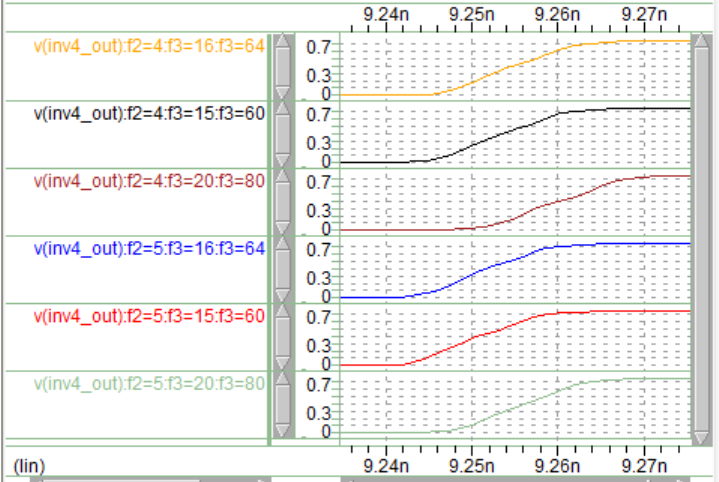
\includegraphics[width=0.9\textwidth]{任务书/image-2.png}
\caption{Rising delay waveforms of inverter chains with different sizing configurations(for illustration only)}
\label{fig:task2_waveform}
\end{figure}

\subsection{Technical Analysis}

The experimental results reveal some important deviations from classical design theory:

For a 4-stage chain with load factor F = 256, the optimal sizing factor should be $f = F^{1/N} = 256^{1/4} = 4$, suggesting uniform scaling with $f_2 = 4, f_3 = 16, f_4 = 64$. However, the practical result is that $f_2 = 5, f_3 = 15, f_4 = 60$, which deviates from the theoretical 4-16-64 progression.

The classical theory assumes identical stage designs with pure capacitive loading. However, in practical FinFET technology, input capacitance includes both gate and parasitic components, while our theory model neglects parasitics capacitance. Moreover, wire parasitic capacitance becomes significant at small feature sizes. That cause drive strength varies non-linearly with transistor sizing. The optimal factor may be slightly larger than 4 (closer to e ≈ 2.718).

\textbf{Stage-by-stage analysis}: 
\begin{itemize}
    \item[1.] Stage 1 and stage 3 shows slightly higher delay with f2=5 vs f2=4 (9.5 ps vs 8.4 ps for stage 1) due to increased load
    \item[2.] Stage 2  and stage 4 benefits significantly from f2=5, showing much lower delay (15.1 ps vs 18.9 ps for stage 2), while the overall delay mainly relies on stage 2 and stage 4 because their larger magnitude.
\end{itemize}


The results demonstrate that practical optimization requires consideration of technology-specific effects beyond simple analytical models.

\newpage
\section{Task 3: CMOS Inverter Power Consumption}

\subsection{Lab Procedures}

Task 3 measures the power consumption of the optimized inverter chain from Task 2. HSPICE simulation is performed with the following key steps:

\begin{enumerate}
    \item[1. ] The optimal sizing configuration: f2 = 5, f3 = 15, f4 = 60
    \item[2. ] A pulse voltage source applied to the input
    \item[3. ] Power measurement averaged over multiple switching cycles
\end{enumerate}

The key HSPICE measurement statement:

\begin{lstlisting}
.measure tran avgpower AVG P(vdd_inv) from=1n to=10n
\end{lstlisting}

This measures the average power consumption from 1 ns to 10 ns, capturing multiple complete switching cycles to obtain accurate steady-state power consumption.

\subsection{Lab Results}

The measured power consumption results are:

\begin{table}[h]
\centering
\begin{tabular}{ccc}
\toprule
\textbf{Parameter} & \textbf{Value} & \textbf{Temperature (°C)} \\
\midrule
Average Power & $-49.86 \mu W$ & 25.0 \\
\bottomrule
\end{tabular}
\caption{Power consumption of optimized inverter chain}
\end{table}

Note: The negative sign indicates power consumption (current flowing from the supply source into the circuit).

\subsection{Technical Analysis}

The power consumption analysis reveals several important characteristics:

\begin{itemize}
    \item[1.] \textbf{Total power}: The measured average power of $-49.86 \mu W$ represents the combined dynamic and static power consumption of the 4-stage inverter chain.
    
    \item[2.] \textbf{Dynamic power dominance}: At nominal supply voltage (0.75V) and room temperature, dynamic switching power typically dominates over static leakage power. The dynamic power is given by:
    $$P_{dynamic} = C_{load} \cdot V_{DD}^2 \cdot P_{0 \rightarrow 1} \cdot f_{clk}$$
    where $P_{0 \rightarrow 1}$ is the activity factor, $C_{load}$ is the total load capacitance, and $f_{clk}$ is the switching frequency.
    
    \item[3.] \textbf{Power-delay trade-off}: While the optimized sizing minimizes delay (37.32 ps), it requires larger transistors in intermediate stages, which increases both switching capacitance and short-circuit current, leading to higher power consumption.
\end{itemize}

These power measurements establish the baseline for energy-delay optimization in Task 4.

\newpage
\section{Task 4: Energy-Delay Product Optimization}

\subsection{Lab Procedures}

Task 4 investigates the optimal operating point ($V_{dd}$) by sweeping supply voltage to minimize the Energy-Delay Product (EDP). The EDP metric captures the trade-off between performance and energy efficiency:

\[EDP = Power \times Delay^2\]

HSPICE simulation is performed with the following key steps:

\begin{enumerate}
    \item[1. ] Use the optimized chain configuration (f2 = 5, f3 = 15, f4 = 60)
    \item[2. ] Sweep supply voltage from 0.5V to 1.5V in 20mV steps
    \item[3. ] Measure total propagation delay ($t_{p\_total}$) for each voltage
    \item[4. ] Measure average power consumption at each voltage
    \item[5. ] Calculate EDP for each operating point
\end{enumerate}

Key HSPICE measurement statements:

\begin{lstlisting}
.measure tran tp_total param='tp1+tp2+tp3+tp4'
.measure TRAN avgpower AVG P(vdd_inv) from=1n to=8n
.measure tran EDP param='abs(avgpower*tp_total*tp_total)'
\end{lstlisting}

A Python script named "parser\_mt.py" was used to extract data from the .mt0 output file and generate visualization plots for analysis.

\subsection{Lab Results}

The simulation swept 51 voltage points from 0.5V to 1.5V. For example, several operating points are summarized in the table below:

\begin{table}[h]
\centering
\begin{tabular}{cccc}
\toprule
\textbf{Supply (V)} & \textbf{$t_{p\_total}$ (ps)} & \textbf{Power ($\mu W$)} & \textbf{EDP ($W \cdot s^2$)} \\
\midrule
0.50 & 44.56 & -20.23 & 4.018×10$^{-26}$ \\
0.56 & 38.60 & -26.20 & 3.904×10$^{-26}$ \\
0.58 & 37.12 & -28.39 & 3.913×10$^{-26}$ \\
0.70 & 31.05 & -43.85 & 4.228×10$^{-26}$ \\
0.80 & 28.12 & -59.85 & 4.732×10$^{-26}$ \\
1.00 & 24.73 & -101.0 & 6.179×10$^{-26}$ \\
1.20 & 22.57 & -617.0 & 31.42×10$^{-26}$ \\
1.50 & 18.80 & -7.093e+6 & 2.507×10$^{-21}$ \\
\bottomrule
\end{tabular}
\caption{Selected EDP measurements at different supply voltages}
\end{table}

The \textbf{optimal supply voltage is 0.56V}, achieving the minimum EDP of \textbf{3.904×10$^{-26} W \cdot s^2$}.

\begin{figure}[htbp]
    \centering
    % 第一张子图
    \begin{subfigure}[b]{0.45\textwidth} % 子图宽度为总宽度的45%
        \centering
        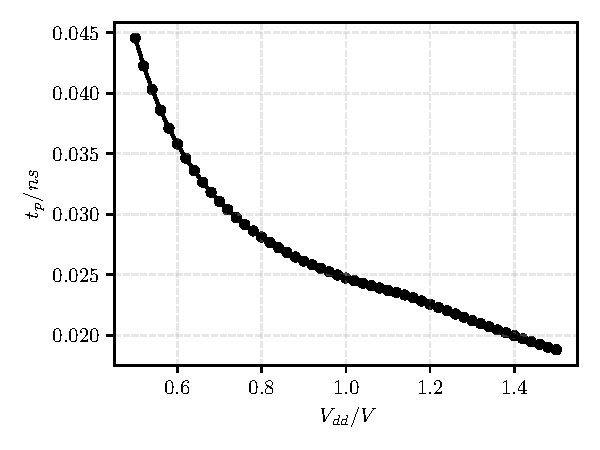
\includegraphics[width=\textwidth]{Task4/tp_total_vs_volts.pdf} 
        \caption{Total propagation delay vs. supply voltage}
        \label{fig:task4_delay}
    \end{subfigure}
    \hfill % 添加水平间距
    % 第二张子图
    \begin{subfigure}[b]{0.45\textwidth}
        \centering
        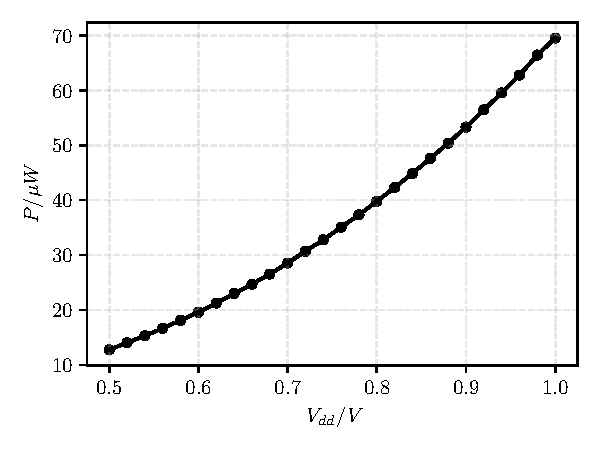
\includegraphics[width=\textwidth]{Task4/power_vs_volts.pdf} 
        \caption{Average power consumption vs. supply voltage}
        \label{fig:task4_power}
    \end{subfigure}
    % 总图标题
    \caption{Delay and Power vs. Supply Voltage}
    \label{fig:task4_delay_power}
\end{figure}

\begin{figure}[h]
\centering
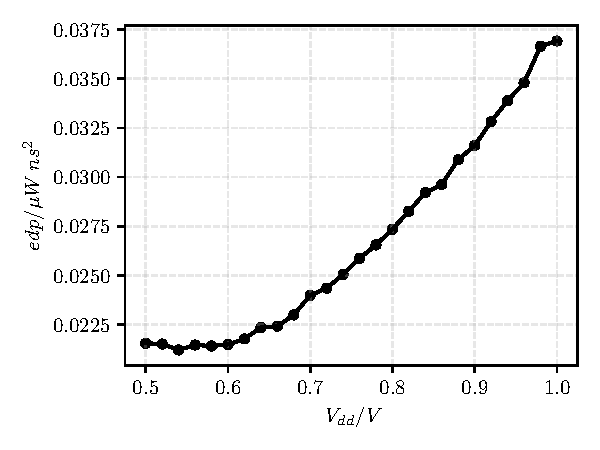
\includegraphics[width=0.75\textwidth]{Task4/edp_vs_volts.pdf}
\caption{Energy-Delay Product vs. supply voltage}
\label{fig:task4_edp}
\end{figure}

\subsection{Technical Analysis}

The voltage scaling results demonstrate fundamental trade-offs in digital circuit design:

\begin{itemize}
    \item[1.] \textbf{Delay characteristics}: As shown in Figure \ref{fig:task4_delay}, delay increases exponentially as supply voltage decreases to threshold. At 0.5V, the circuit operates near the threshold voltage region where transistor drive current is severely degraded.
    
    \item[2.] \textbf{Power characteristics}: Figure \ref{fig:task4_power} shows that power consumption decreases quadratically with supply voltage, following the relationship $P \propto V_{DD}^2$. At 1.0V, power is 69.53 $\mu W$, while at 0.58V it drops to 18.12 $\mu W$ (a 74\% reduction).
    
    \item[3.] \textbf{EDP optimization}: Figure \ref{fig:task4_edp} reveals a minimum at 0.58V. This represents the optimal balance between:
    \begin{itemize}
        \item Speed: Still reasonable at 34.37 ps ( 49\% slower than at 1.0V)
        \item Energy efficiency: Power reduced by 74\% compared to nominal voltage
    \end{itemize}
    
\end{itemize}

The EDP metric effectively captures the energy-performance trade-off, making it a valuable tool for system-level power management decisions.

\newpage
\section{Task 5: Inverter Chain Optimization with Unfixed Stages}

\subsection{Lab Procedures}

Task 5 extends the optimization problem by allowing the number of stages ($N$) to vary. The goal is to find both the optimal number of stages and the sizing factor for each stage to minimize total delay.

Theoretical background:
\begin{itemize}
    \item For a given stage number $N$, the optimal sizing factor is $f = F^{1/N}$ where F = 256 (load factor)
    \item If $N$ is not given, the optimal number of stages should satisfy: $f = \exp(1 + \gamma/f) \approx 3.6$ (from calculus of variations)
    \item This suggests N = $\ln(256)/\ln(3.6) \approx 4.32$ stages
\end{itemize}

HSPICE simulation is performed with the following key steps:
\begin{enumerate}
    \item[1. ] Generate separate HSPICE netlists for N = 1 to 10 stages
    \item[2. ] For each N, calculate optimal sizing as $f = 256^{1/N}$
    \item[3. ] Use Python scripts to automatically generate netlists and batch simulate
    \item[4. ] Extract total delay for each configuration
    \item[5. ] Compare results to identify optimal stage number
\end{enumerate}

Python  scripts used for automation work are:
\begin{itemize}
    \item[1. ] \texttt{generate\_task5.py}: Generates HSPICE netlists for different N values
    \item[2. ] \texttt{run\_task5.py}: Batch executes all simulations
    \item[3. ] \texttt{parser\_mt.py}: Parses .mt0 output files
    \item[4. ] \texttt{run\_stat.py}: Consolidates results into summary spreadsheet
    \item[5. ] \texttt{summary\_plot.py}: Generates visualization plots
\end{itemize}

\subsection{Lab Results}

The simulation results for stage numbers from 1 to 10 are summarized:

\begin{table}[h]
\centering
\begin{tabular}{ccc}
\toprule
\textbf{N (Stages)} & \textbf{$t_{p\_total}$ (ps)} & \textbf{Optimal f} \\
\midrule
1 & 208.8 & 256.00 \\
2 & 46.43 & 16.00 \\
3 & 31.96 & 6.35 \\
4 & 29.63 & 4.00 \\
5 & 29.12 & 3.03 \\
6 & 30.34 & 2.52 \\
7 & 31.82 & 2.20 \\
8 & 33.02 & 1.97 \\
9 & 34.87 & 1.81 \\
10 & 36.95 & 1.68 \\
\bottomrule
\end{tabular}
\caption{Total delay vs. number of stages}
\end{table}

The \textbf{optimal configuration is N = 5 stages} with a minimum total delay of \textbf{29.12 ps}.

\begin{figure}[h]
\centering
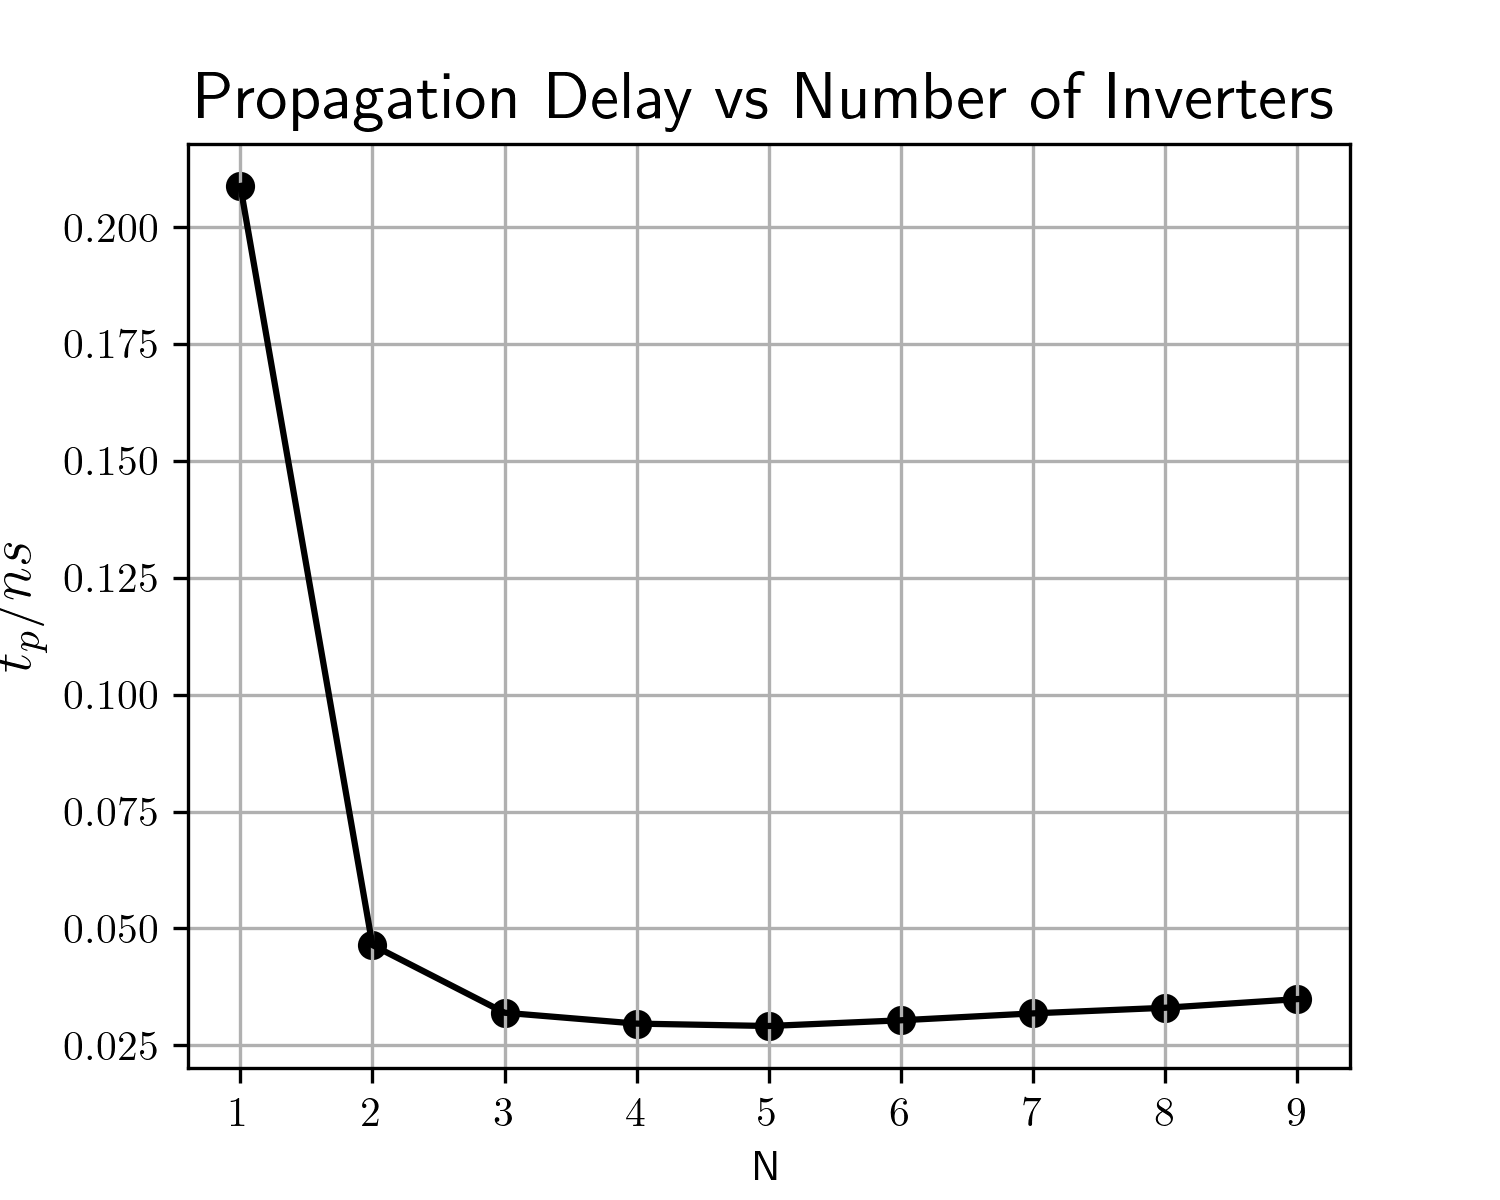
\includegraphics[width=0.8\textwidth]{Task5/tp_N.png}
\caption{Total propagation delay vs. number of stages}
\label{fig:task5_delay}
\end{figure}

\subsection{Technical Analysis}

The results validate theoretical predictions and reveal practical design insights:

\begin{itemize}
    \item[1. ] \textbf{Optimal stage number}: The experimental optimum of N = 5 closely matches the theoretical prediction of $N \approx 4.32$ stages. This confirms that the optimal sizing factor should be near $f \approx 3.6$. At N = 5, $f = 256^{1/5} = 3.03$, which is reasonably close to 3.6.

    \item[2. ] \textbf{Delay vs. stages curve}: Figure \ref{fig:task5_delay} shows a minimum at N = 5:
    \begin{itemize}
        \item N < 5: Too few stages means each stage must provide large gain, resulting in excessive delay per stage
        \item N > 5: Too many stages accumulate delay despite each being individually fast
        \item N = 5: Optimal balance between stage count and individual stage delay
    \end{itemize}
    
    \item[3. ] \textbf{Single stage penalty}: Using just 1 stage (N=1) results in 208.8 ps delay - over 7× slower than the optimum. This dramatic penalty demonstrates why direct drive of large loads is impractical.
    
    \item[4. ] \textbf{Diminishing returns}: The delay reduction from N=4 to N=5 is 0.51 ps (1.7\% improvement), while further increasing stages degrades performance. This suggests the optimization landscape is relatively flat near the optimum, which provides design flexibility.
    
    \item[5. ] \textbf{Comparison with Task 2}: 
    \begin{itemize}
        \item Task 2 (fixed 4 stages): Best delay = 37.32 ps
        \item Task 5 (optimized 5 stages): Delay = 29.12 ps
        \item Improvement: 22\% faster by adding one stage and optimizing sizing
    \end{itemize}


    \item \textbf{Technology scaling}: The optimal $N$ depends on the ratio of intrinsic delay to loading delay. As technology scales to smaller nodes with lower supply voltages, this ratio changes, potentially shifting the optimal $N$.
\end{itemize}

This task demonstrates the importance of holistic optimization - considering both stage count and transistor sizing to achieve optimal circuit performance.

\newpage
\section{Observations and Conclusions}

This laboratory investigation of CMOS inverter chains using 16nm FinFET technology has provided valuable insights into fundamental digital circuit design principles and optimization techniques.

\subsection{Key Observations}

\begin{enumerate}
    \item \textbf{FO4 Delay Characterization}: The measured FO4 delay of 5.9 ps demonstrates the high-speed capability of advanced FinFET technology. The slight asymmetry between $t_{pLH}$ and $t_{pHL}$ (9\% difference) reflects inherent mobility differences between NMOS and PMOS devices.

    \item \textbf{Theoretical vs. Practical Optimization}: While classical theory predicts uniform 4× scaling for optimal delay, experimental results show that $f_2=5, f_3=15, f_4=60$ provides superior performance. This deviation highlights the importance of parasitic effects, non-ideal scaling, and technology-specific characteristics that simple analytical models may overlook.
    
    \item \textbf{Voltage Scaling for Energy Efficiency}: The EDP analysis revealed that operating at 0.58V (27\% below nominal) achieves optimal energy efficiency. This represents a 74\% power reduction with only 49\% delay penalty, making it highly attractive for energy-constrained applications.
    
    \item \textbf{Architectural Optimization}: Allowing variable stage count (Task 5) achieved 22\% better performance compared to fixed 4-stage design (Task 2). The optimal $N=5$ stages with $f \approx 3.03$ validates theoretical predictions based on $f = 3.6$.
\end{enumerate}

\subsection{Conclusions}

\begin{enumerate}
    \item \textbf{Multi-dimensional optimization}: Optimal circuit design requires simultaneous consideration of multiple parameters - transistor sizing, stage count, and supply voltage. No single parameter can be optimized in isolation without considering its impact on other design objectives.
    
    \item \textbf{Technology awareness}: Practical design must account for real-world effects including parasitic capacitance, wire resistance, velocity saturation, and short-channel effects, which becomes increasingly important at advanced technology nodes.
    
    \item \textbf{Design metrics matter}: Different optimization metrics (minimum delay, minimum power, minimum EDP) lead to different optimal designs:
    \begin{itemize}
        \item Minimum delay: Large transistors, nominal voltage, optimal staging
        \item Minimum power: Small transistors, reduced voltage
        \item Minimum EDP: Balanced sizing, near-threshold voltage
    \end{itemize}
\end{enumerate}

In conclusion, this lab has successfully demonstrated the application of systematic optimization techniques to inverter chain design, validating theoretical models while revealing the importance of practical considerations in advanced technology nodes. The methodologies and insights gained are directly applicable to real-world digital circuit design problems.

\end{document}
